\documentclass[a4paper, 12pt]{ctexart}
\usepackage[UTF8]{ctex}
\usepackage{amsmath}
\usepackage{graphicx}
\usepackage{grffile}
\usepackage{longtable}
\usepackage{wrapfig}
\usepackage{rotating}
\usepackage{cases}
\usepackage{mathrsfs}
\usepackage{amssymb} 
\usepackage{amsthm}
\usepackage{xltxtra} 
\usepackage{mflogo,texnames}
\usepackage{indentfirst}
\usepackage[normalem]{ulem}
\usepackage{textcomp}
\usepackage{booktabs}
\usepackage{subfigure}
\usepackage{caption}
\usepackage[linktocpage,pdfstartview=FitH,colorlinks,
linkcolor=blue,anchorcolor=blue,
citecolor=blue,filecolor=blue,menucolor=blue,urlcolor=blue]{hyperref}
\usepackage{setspace,csquotes, enumitem,endnotes,fontspec, capt-of}
\doublespacing
\usepackage[margin=1in]{geometry}
\usepackage[notes, notetype=endonly, isbn=false, backend=biber]{biblatex-chicago}
\bibliography{shiff2016b}
\let\footnote=\endnote
\let\cite=\endnote
\let\footcite=\autocite
\setCJKmainfont{SimSun}
\setmainfont{Calibri} 
\CTEXsetup[format={\Large\bfseries}]{section}
\setlist[enumerate,itemize]{noitemsep,nolistsep,leftmargin=*}
\newtheorem*{theorem}{解}
\newtheorem*{example}{问题}
\usepackage{listings}
\usepackage[usenames,dvipsnames]{color}
\definecolor{DarkGreen}{rgb}{0.0,0.4,0.0}
\lstloadlanguages{Matlab}
\lstset{language=Matlab,
        % frame=single,                           % single framed
        basicstyle=\small,
        keywordstyle=[1]\color{Blue}\bfseries,  % primitive funs in bold blue
        keywordstyle=[2]\color{Purple},         % args of funs in purple
        keywordstyle=[3]\color{Blue}\underbar,  % user funs in blue with underbar
        stringstyle=\color{Purple},             % strings in purple
        showstringspaces=false,
        identifierstyle=,
        tabsize=4,
        % more standard MATLAB funcs
        morekeywords={sawtooth, square},
        % args of funcs
        morekeywords=[2]{on, off, interp},
        % user funcs
        morekeywords=[3]{FindESS, homework_example},
        morecomment=[l][\color{Blue}]{...},     % line continuation (...) like blue comment
        numbers=left,
        numberstyle=\tiny\color{Blue},
        firstnumber=1,
        stepnumber=1
        }


\author{张天骏 \\ 2021300003004}
\date{}
\title{MATLAB及其应用结课报告}


\begin{document}
\maketitle

\section{题目描述}

一个空间移动目标沿曲线$L$运动,其关于时间$t$(时间单
位:秒,坐标单位:米),的参数方程如下:

$$\begin{cases}
    x_1(t)=a+bt+A\cos \omega_1 t \\
    y_1(t)=c+dt+B\sin \omega_2 t \\
    z_1(t)=e+C\sin \omega_3 t
\end{cases}$$

其中$a,b,c,d,e,A,B,C,\omega_1,\omega_2,\omega_3$是常数。
在$t=0$的时候
突然被位于坐标$(0,0,0)$点探测器发现并锁定,随即发射跟踪器且以恒定速率($v$ 米/秒)
追击移动目标,且追击方向始终指向移动目标,如下图所示:

\begin{figure}[h]
    \centering
    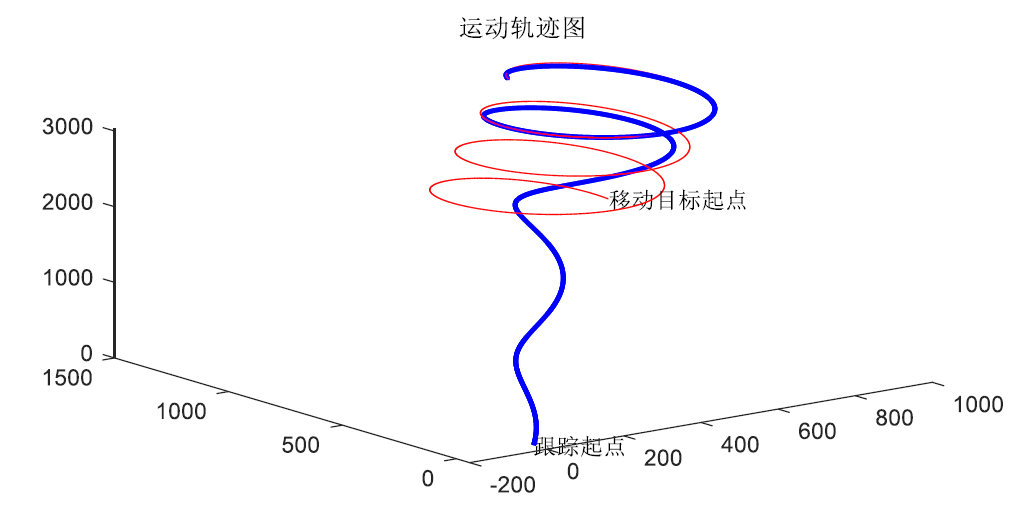
\includegraphics[width=0.8\linewidth]{pic/1.png}
\end{figure}


\section{题目解决}

\subsection{第一题}

\begin{example}
    请根据附件中给出的空间移动目标随时间移动的空间位置数据文件(数据文件名
    data1.txt,数据格式$[t,x_1(t),y_1(t),z_1(t)]$),预估移动目标的最大速度和最小速度;
\end{example}

\begin{theorem}
直接读取数据可以得到:最大速度: 402.599591 米/秒,最小速度: 157.141857 米/秒
\begin{lstlisting}
%% 第一题
% 读取数据
data1 = load('data1.txt'); % 假设文件格式为 [t, x, y, z]
t1 = data1(:, 1);
x1 = data1(:, 2);
y1 = data1(:, 3);
z1 = data1(:, 4);
% 计算速度
dt = diff(t1);
dx = diff(x1);
dy = diff(y1);
dz = diff(z1);
speed = sqrt((dx./dt).^2 + (dy./dt).^2 + (dz./dt).^2);
% 找到最大和最小速度
max_speed = max(speed);
min_speed = min(speed);
fprintf('最大速度: %f 米/秒\n', max_speed);
fprintf('最小速度: %f 米/秒\n', min_speed);
\end{lstlisting}
\end{theorem}

%%%%%%%%%%%%%%%%%%%%%%%%%%%%%%%%%%%%%%%%%%%%%%%%%%%%%%%%%%
\subsection{第二题}

\begin{example}
    请根据附件中给出的空间移动目标随时间移动的空间位置数据文件(数据文件名
    data1.txt,数据格式$[t,x_1(t),y_1(t),z_1(t)]$),
    确定空间移动目标曲线$L$中的待定常数$a,b,c,d,e,A,B,C,\omega_1,\omega_2,\omega_3$
    。画出空间移动目标在$t\in [0,20]$变化的轨迹图、速度图,并求出速度的最大和最小值
\end{example}

\begin{theorem}
    我首先画出了三个位置分量$(x(t),y(t),z(t))$关于$t$的图像,以此为依据进行非线性拟合。
    根据$(t,x(t))$的图像特征,我对于参数$A,\omega_1$做出以下约束:$150<A<300,\pi/4 < \omega_1 < \pi/2$
    。我的依据是:图像两个极大值点的间距在4到8之间,可以推断$4<T=2\pi / \omega_1 <8$;图像的极差在400左右,
    可以估计$A$在200左右取值。
    \begin{lstlisting}
% 设置 fittype 和选项。
ft = fittype( 'a+b*x+c*cos(d*x)', 'independent', 'x', ...
    'dependent', 'y' );
opts = fitoptions( 'Method', 'NonlinearLeastSquares' );
opts.Display = 'Off';
opts.Lower = [-Inf -Inf 150 0.75];
opts.StartPoint = [0.149 0.257 0.840 0.254];
opts.Upper = [Inf Inf 300 1.5];
% 对数据进行模型拟合。
[fitresult_x, gof] = fit( t1, x1, ft, opts );
% 绘制数据拟合图。
figure( 'Name', 'x 拟合' );
h = plot( fitresult_x, t1, x1 );
legend( h, '原始数据', '拟合结果', 'Location', 'NorthEast', ...
    'Interpreter', 'none' );
% 为坐标区加标签
xlabel( 't1', 'Interpreter', 'none' );
ylabel( 'x1', 'Interpreter', 'none' );
grid on
    \end{lstlisting}
    根据类似的想法,可以得到$(t,y(t))$的拟合代码:
    \begin{lstlisting}
% 设置 fittype 和选项。
ft = fittype( 'a+b*x+c*sin(d*x)', 'independent', 'x', ...
    'dependent', 'y' );
opts = fitoptions( 'Method', 'NonlinearLeastSquares' );
opts.Display = 'Off';
opts.Lower = [-Inf -Inf 300 0.75];
opts.StartPoint = [0.890 0.959 0.547 0.138];
opts.Upper = [Inf Inf 500 1.5];
% 对数据进行模型拟合。
[fitresult_y, gof] = fit( t1, y1, ft, opts );
% 绘制数据拟合图。
figure( 'Name', '拟合 y' );
h = plot( fitresult_y, t1, y1 );
legend( h, '原始数据', '拟合结果', 'Location', 'NorthEast', ...
    'Interpreter', 'none' );
% 为坐标区加标签
xlabel( 't1', 'Interpreter', 'none' );
ylabel( 'y1', 'Interpreter', 'none' );
grid on
    \end{lstlisting}
    而至于$(t,z(t))$的拟合,注意到图像在$[0,20]$是单调递增的,所以可以得到条件$\pi/2\omega_3=T/4 > 20$
    从而有$0< \omega_3 < \pi/40$,基于此可以得到拟合代码:
    \begin{lstlisting}
% 设置 fittype 和选项。
ft = fittype( 'a+b*sin(c*x)', 'independent', 'x', ...
    'dependent', 'y' );
opts = fitoptions( 'Method', 'NonlinearLeastSquares' );
opts.Display = 'Off';
opts.Lower = [-Inf 0 0];
opts.StartPoint = [0.162611735194631 0.118997681558377 1];
opts.Upper = [Inf Inf 0.078];

% 对数据进行模型拟合。
[fitresult_z, gof] = fit( t1, z1, ft, opts );

% 绘制数据拟合图。
figure( 'Name', '拟合 z' );
h = plot( fitresult_z, t1, z1 );
legend( h, '真实数据', '拟合结果', 'Location', 'NorthEast', ...
    'Interpreter', 'none' );
% 为坐标区加标签
xlabel( 't', 'Interpreter', 'none' );
ylabel( 'z', 'Interpreter', 'none' );
grid on
    \end{lstlisting}
    最终分量的拟合结果图如下:
    \begin{figure}[h]
        \centering
        \nonumber
        \subfigure{
        \begin{minipage}[t]{0.32\linewidth}
        \centering
        \nonumber
        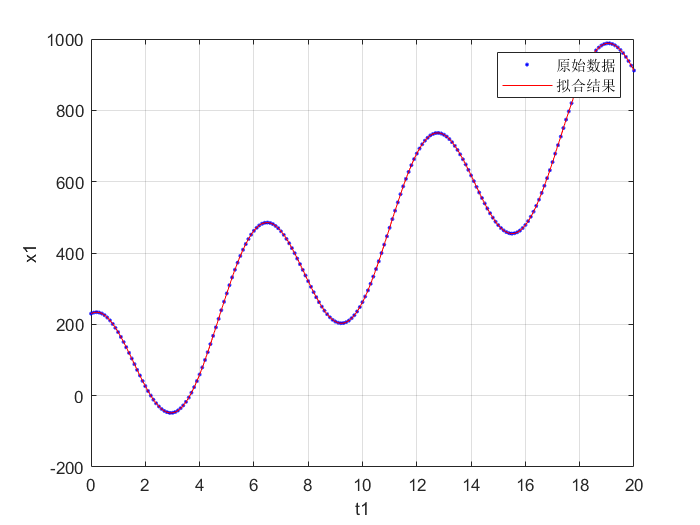
\includegraphics[width=2in]{pic/fit_x.png}
        \caption*{x分量拟合}
        \end{minipage}}
        \subfigure{
        \begin{minipage}[t]{0.32\linewidth}
        \centering
        \nonumber
        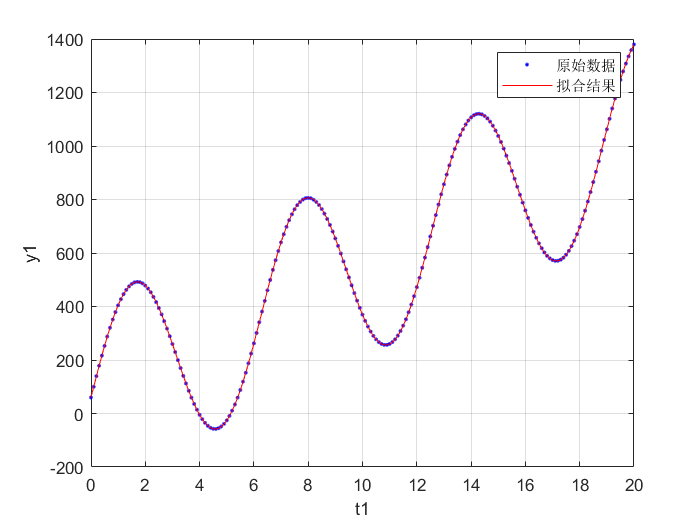
\includegraphics[width=2in]{pic/fit_y.png}
        \caption*{y分量拟合}
        \end{minipage}}
        \subfigure{
        \begin{minipage}[t]{0.32\linewidth}
        \centering
        \nonumber
        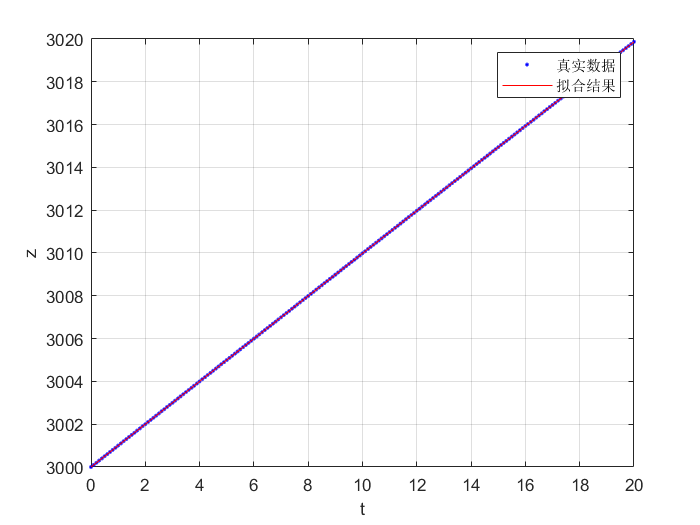
\includegraphics[width=2in]{pic/fit_z.png}
        \caption*{z分量拟合}
        \end{minipage}}
    \end{figure}
    接下来,我们基于上面的拟合结果确定常数$a,b,c,d,e,A,B,C,\omega_1,\omega_2,\omega_3$
    求解拟合的速度极值:
    \begin{lstlisting}
a = fitresult_x.a;
b = fitresult_x.b;
A = fitresult_x.c;
w1 = fitresult_x.d;
c = fitresult_y.a;
d = fitresult_y.b;
B = fitresult_y.c;
w2 = fitresult_y.d;
e = fitresult_z.a;
C = fitresult_z.b;
w3 = fitresult_z.c;
fitted_x = a + b*t1 + A*cos(w1*t1);
fitted_y = c + d*t1 + 350*sin(w2*t1);
fitted_z = e + C*sin(w3*t1);
figure;
plot3(x1, y1, z1, 'r.', fitted_x, fitted_y, fitted_z, 'b-');
xlabel('x'); ylabel('y'); zlabel('z');
title('运动轨迹拟合');
legend('原始数据', '拟合曲线', 'Location', 'best');
grid on;
% 计算速度
speed_fit = sqrt((b-A*w1*sin(w1*t1)).^2 + ...
    (d+B*w2*cos(w2*t1)).^2 + ...
    ((C*w3*cos(w3*t1)).^2));
% 绘制速度图
figure;
plot(t1, speed_fit, 'b-');
xlabel('时间 (秒)');
ylabel('速度 (米/秒)');
title('速度图');
grid on;
% 最大和最小速度
max_speed_fit = max(speed_fit);
min_speed_fit = min(speed_fit);
fprintf('拟合最大速度: %f 米/秒\n', max_speed_fit);
fprintf('拟合最小速度: %f 米/秒\n', min_speed_fit);
    \end{lstlisting}
    \begin{figure}[h]
        \centering
        \nonumber
        \subfigure{
        \begin{minipage}[t]{0.45\linewidth}
        \centering
        \nonumber
        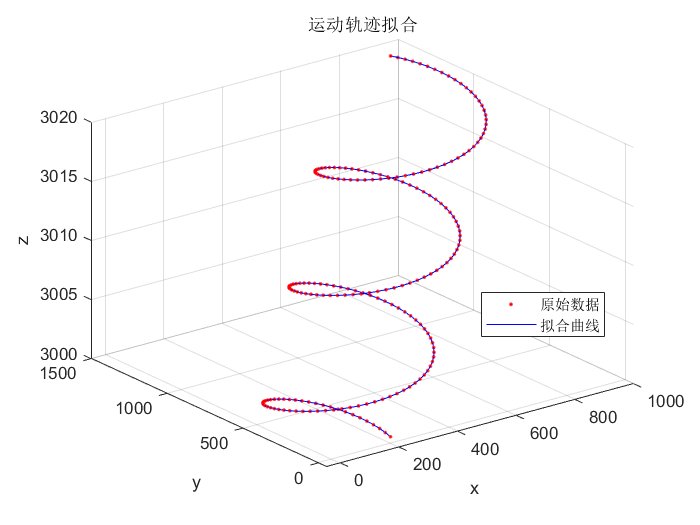
\includegraphics[width=3in]{pic/fit.png}
        \end{minipage}}
        \subfigure{
        \begin{minipage}[t]{0.45\linewidth}
        \centering
        \nonumber
        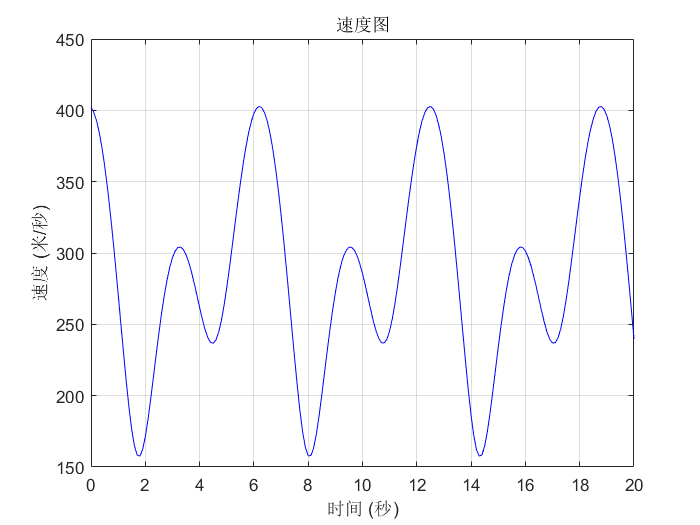
\includegraphics[width=3in]{pic/fit_speed.png}
        \end{minipage}}
    \end{figure}
    拟合最大速度: 402.790059 米/秒,拟合最小速度: 157.501787 米/秒
\end{theorem}
%%%%%%%%%%%%%%%%%%%%%%%%%%%%%%%%%%%%%%%%%%%%%%%%%%%%%%%%%%
\subsection{第三题}

\begin{example}
    证明跟踪器的运动轨迹$(x(t),y(t),z(t))$满足如下微分方程组的初始问题,并当跟
    踪器运动速度$v=300$ 米/秒 时,数值求解微分方程组,并
    画出空间移动目标在$t\in [0,20]$变化的轨迹图、速度图,并求出速度的最大和最小值
    $$\begin{cases}
    \frac{dx(t)}{dt} = \frac{v}{\sqrt{(x_1(t)-x(t))^2+(y_1(t)-y(t))^2+(z_1(t)-z(t))^2}} (x_1(t)-x(t))  \\
    \frac{dy(t)}{dt} = \frac{v}{\sqrt{(x_1(t)-x(t))^2+(y_1(t)-y(t))^2+(z_1(t)-z(t))^2}} (y_1(t)-y(t))  \\
    \frac{dz(t)}{dt} = \frac{v}{\sqrt{(x_1(t)-x(t))^2+(y_1(t)-y(t))^2+(z_1(t)-z(t))^2}} (z_1(t)-z(t))  \\
    x(0)=y(0)=z(0)=0
    \end{cases}
    $$
\end{example}


\begin{proof}
    首先,根据追踪器的特性,追踪器在$t$时刻的速度方向一定是追踪器位置和目标位置的连线,指向目标。
    在$t$时刻,追踪器位置为$(x(t),y(t),z(t))$,目标位置为$(x_1(t),y_1(t),z_1(t))$,
    二者连线,指向目标的单位向量为$\frac{(x_1(t)-x(t),y_1(t)-y(t),z_1(t)-z(t))}{\sqrt{(x_1(t)-x(t))^2+(y_1(t)-y(t))^2+(z_1(t)-z(t))^2}}$
    对$t$时刻追踪器速度$v$依据该向量正交分解,便可以得到上述微分方程组
\end{proof}



\begin{theorem}
    根据题干和证明建立微分方程组模型,使用ode45包进行数值求解:
\begin{lstlisting}
%% 第三题
% 微分方程的初值问题
v_3 = 300; % 跟踪器速度
% 建立微分方程组
% target_trajectory = @(t)[a + b*t+A*cos(w1*t); ...
                           c + d*t+B*sin(w2*t); ...
                           e + C*sin(w3*t)];
tracker_ode_3 = @(t, y)[
v_3*(a+b*t+A*cos(w1*t) -y(1)) / sqrt((a+b*t+A*cos(w1*t)-y(1)).^2 ...
+ (c+d*t+B*sin(w2*t)-y(2)).^2+(e+C*sin(w3*t)-y(3)).^2);
v_3*(c+d*t+B*sin(w2*t)-y(2)) / sqrt((a+b*t+A*cos(w1*t)-y(1)).^2 ...
+ (c+d*t+B*sin(w2*t)-y(2)).^2+(e + C*sin(w3*t)-y(3)).^2);
v_3*(e+C*sin(w3*t) -y(3)) / sqrt((a+b*t+A*cos(w1*t)-y(1)).^2 ...
+(c+d*t+B*sin(w2*t)-y(2)).^2+(e+C*sin(w3*t)-y(3)).^2)
];
% 初始条件
y0 = [0; 0; 0];
% 时间跨度
tspan = [0 20];
% 求解微分方程
[t_sol_3, y_sol_3] = ode45(tracker_ode_3, tspan, y0);
% 绘制跟踪器和目标的轨迹图
figure;
plot3(x1, y1, z1, 'r-', ...
    y_sol_3(:, 1), y_sol_3(:, 2), y_sol_3(:, 3), 'b-');
xlabel('x');
ylabel('y');
zlabel('z');
title('移动目标和跟踪器的轨迹');
legend('目标轨迹', '跟踪器轨迹');
grid on;
\end{lstlisting}
\begin{figure}[h]
    \centering
    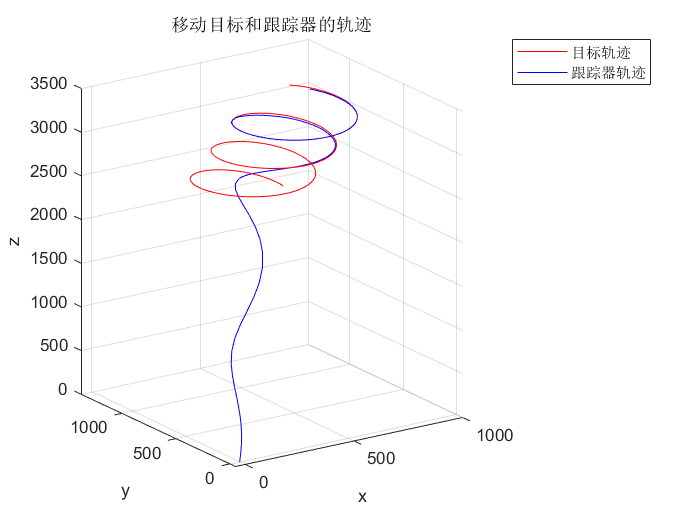
\includegraphics[width=4.5in]{pic/t3.png}
    \caption*{第三题轨迹}
\end{figure}

\end{theorem}







%%%%%%%%%%%%%%%%%%%%%%%%%%%%%%%%%%%%%%%%%%%%%%%%%%%%%%%%%%
\subsection{第四题}

\begin{example}
    当速度 $v=290$ 米/秒 时,在30秒时间内,跟踪器能否追上移动目标? 若能追上,
    需多长时间?并画出跟踪器和移动目标的运动轨迹图
\end{example}


\begin{theorem}
    同理第三问求解微分方程组,并计算每个取点下追踪器和目标之间的距离,定义距离小于1米为追上:
\begin{lstlisting}
%% 第四题
% 跟踪器速度
v_4 = 290; % 米/秒
% 求解微分方程
tracker_ode_4 = @(t, y)[
v_4*(a+b*t+A*cos(w1*t) -y(1)) / sqrt((a+b*t+A*cos(w1*t)-y(1)).^2 ...
+ (c+d*t+B*sin(w2*t)-y(2)).^2+(e+C*sin(w3*t)-y(3)).^2);
v_4*(c+d*t+B*sin(w2*t)-y(2)) / sqrt((a+b*t+A*cos(w1*t)-y(1)).^2 ...
+ (c+d*t+B*sin(w2*t)-y(2)).^2+(e + C*sin(w3*t)-y(3)).^2);
v_4*(e+C*sin(w3*t) -y(3)) / sqrt((a+b*t+A*cos(w1*t)-y(1)).^2 ...
+(c+d*t+B*sin(w2*t)-y(2)).^2+(e+C*sin(w3*t)-y(3)).^2)
];
[t_sol_4, y_sol_4] = ode45(tracker_ode_4, [0 30], [0;0;0]);
% 计算距离
distance_4 = sqrt((y_sol_4(:,1)-a-b*t_sol_4-A*cos(w1*t_sol_4)).^2+ ...
                (y_sol_4(:,2)-c-d*t_sol_4-B*sin(w2*t_sol_4)).^2+ ...
                (y_sol_4(:,3)-e-C*sin(w3*t_sol_4)).^2);
% 判断是否追上
if any(distance_4 < 1) % 假设追上条件为距离小于1米
    fprintf('跟踪器在 %f 秒时追上目标\n', ...
        t_sol_4(find(distance_4 < 1, 1)));
else
    fprintf('跟踪器在 30 秒内未能追上目标\n');
end
% 绘制轨迹图
figure;
plot3(x1, y1, z1, 'r-', ...
    y_sol_4(:, 1), y_sol_4(:, 2), y_sol_4(:, 3), 'b-');
xlabel('x');
ylabel('y');
zlabel('z');
title('移动目标和跟踪器的轨迹');
legend('目标轨迹', '跟踪器轨迹');
grid on;
\end{lstlisting}
\begin{figure}[h]
    \centering
    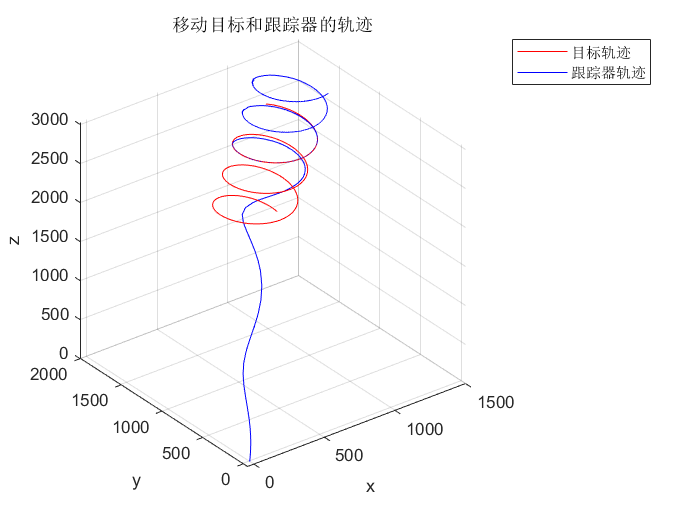
\includegraphics[width=5in]{pic/t4.png}
    \caption*{第四题轨迹}
\end{figure}
结论:跟踪器在 30 秒内未能追上目标
\end{theorem}
%%%%%%%%%%%%%%%%%%%%%%%%%%%%%%%%%%%%%%%%%%%%%%%%%%%%%%%%%%
\subsection{第五题}

\begin{example}
    当速度 $v=200$ 米/秒 时,在30秒时间内,跟踪器能否追上移动目标? 若能追上,
    需多长时间?并画出跟踪器和移动目标的运动轨迹图
\end{example}

\begin{theorem}
    同理第四问,只需要将速度改为200米/秒:
\begin{lstlisting}
%% 第四题
% 跟踪器速度
v_5 = 200; % 米/秒
% 求解微分方程
tracker_ode_5 = @(t, y)[
v_5*(a+b*t+A*cos(w1*t) -y(1)) / sqrt((a+b*t+A*cos(w1*t)-y(1)).^2 ...
+ (c+d*t+B*sin(w2*t)-y(2)).^2+(e+C*sin(w3*t)-y(3)).^2);
v_5*(c+d*t+B*sin(w2*t)-y(2)) / sqrt((a+b*t+A*cos(w1*t)-y(1)).^2 ...
+ (c+d*t+B*sin(w2*t)-y(2)).^2+(e + C*sin(w3*t)-y(3)).^2);
v_5*(e+C*sin(w3*t) -y(3)) / sqrt((a+b*t+A*cos(w1*t)-y(1)).^2 ...
+(c+d*t+B*sin(w2*t)-y(2)).^2+(e+C*sin(w3*t)-y(3)).^2)
];
[t_sol_5, y_sol_5] = ode45(tracker_ode_4, [0 30], [0;0;0]);
% 计算距离
distance_5 = sqrt((y_sol_5(:,1)-a-b*t_sol_5-A*cos(w1*t_sol_5)).^2+ ...
                (y_sol_5(:,2)-c-d*t_sol_5-B*sin(w2*t_sol_5)).^2+ ...
                (y_sol_5(:,3)-e-C*sin(w3*t_sol_5)).^2);
% 判断是否追上
if any(distance_5 < 1) % 假设追上条件为距离小于1米
    fprintf('跟踪器在 %f 秒时追上目标\n', ...
        t_sol_5(find(distance_5 < 1, 1)));
else
    fprintf('跟踪器在 30 秒内未能追上目标\n');
end
% 绘制轨迹图
figure;
plot3(x1, y1, z1, 'r-', ...
    y_sol_5(:, 1), y_sol_5(:, 2), y_sol_5(:, 3), 'b-');
xlabel('x');
ylabel('y');
zlabel('z');
title('移动目标和跟踪器的轨迹');
legend('目标轨迹', '跟踪器轨迹');
grid on;
\end{lstlisting}
\begin{figure}[h]
    \centering
    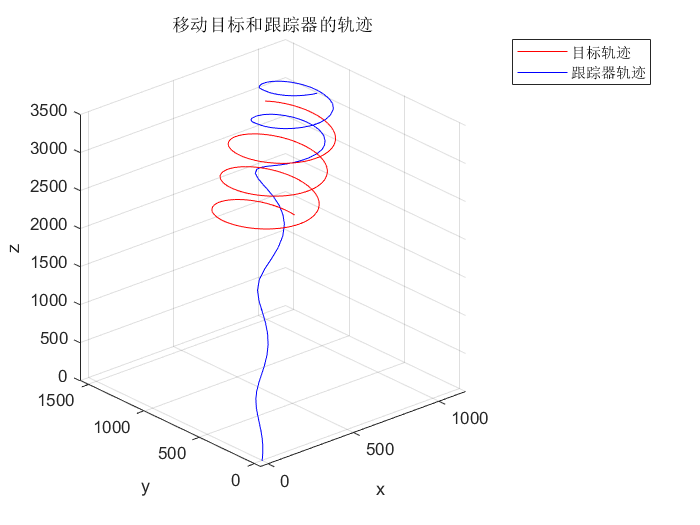
\includegraphics[width=5in]{pic/t5.png}
    \caption*{第五题轨迹}
\end{figure}
结论:跟踪器在 30 秒内未能追上目标
\end{theorem}
%%%%%%%%%%%%%%%%%%%%%%%%%%%%%%%%%%%%%%%%%%%%%%%%%%%%%%%%%%
\subsection{第六题}

\begin{example}
    若要使跟踪器在30秒内追上移动目标,问至少需要多大的追击速度$v$ ,并求从$t=0$
    开始追击到追上目标,并求所花费的时间和各自行进的轨迹长度;
\end{example}

\begin{theorem}
    通过遍历速度范围,逐步增加初始速度来寻找追踪器在30秒内追上目标的最小速度。
    目标位置由参数化函数表示,代码在每次迭代中计算追踪器与目标在各个时间点的距
    离,若距离小于1米,则认为追上目标并记录当前速度和追击时间。找到合适速度后,
    输出追踪器和目标的行进轨迹,并计算两者的轨迹长度。第一次我选择步长为1米/秒
    锁定目标范围,然后缩小搜索范围并换步长为0.01 米/秒,最终得到了比较精确的结果。
    \begin{lstlisting}
% 目标位置的函数,假设从问题二中得到的参数已定义
targetX = @(t) a + b*t + A*cos(w1*t);
targetY = @(t) c + d*t + B*sin(w2*t);
targetZ = @(t) e + C*sin(w3*t);
% 设置初始速度范围
v_min = 0; % 初始速度
v_max = 400; % 假设最大速度为400米/秒
v_increment = 1; % 每次增加1米/秒
% 初始条件和时间区间
w0 = [0; 0; 0];
tspan = [0 30];
% 迭代寻找最小速度
for v = v_min:v_increment:v_max
    odefun = @(t, w) [v * (targetX(t) - w(1)) / sqrt((targetX(t) - ...
                     w(1))^2 + (targetY(t) - w(2))^2 + (targetZ(t) - ... 
                     w(3))^2);
                     v * (targetY(t) - w(2)) / sqrt((targetX(t) - ...
                     w(1))^2 + (targetY(t) - w(2))^2 + (targetZ(t) - ...
                     w(3))^2);
                     v * (targetZ(t) - w(3)) / sqrt((targetX(t) - ...
                     w(1))^2 + (targetY(t) - w(2))^2 + (targetZ(t) - ...
                     w(3))^2)];
    [t, w] = ode45(odefun, tspan, w0);
    % 计算每一时间点上的距离
    distances = sqrt((targetX(t) - w(:,1)).^2 + (targetY(t) - ...
                w(:,2)).^2 + (targetZ(t) - w(:,3)).^2);
    % 检查是否追上
    if any(distances < 1) % 假设追上的条件是距离小于1米
        idx = find(distances < 1, 1, 'first');
        catch_time = t(idx);
        fprintf('最小追击速度: %.2f 米/秒\n', v);
        fprintf('追踪器在 %.2f 秒内追上了目标。\n', catch_time);
        break; % 找到最小速度后跳出循环
    end
end
if v == v_max
    fprintf('在最大速度 %d 米/秒内追踪器未能在30秒内追上目标。\n', v_max);
end

%% 进一步搜索
v_min = 292; % 更换最小速度
v_max = 294; % 更换最大速度
v_increment = 0.01; % 每次增加0.01米/秒
% 初始条件和时间区间
w0 = [0; 0; 0];
tspan = [0 30];
% 迭代寻找最小速度
for v = v_min:v_increment:v_max
    odefun = @(t, w) [v * (targetX(t) - w(1)) / sqrt((targetX(t) - ...
                     w(1))^2 + (targetY(t) - w(2))^2 + (targetZ(t) - ... 
                     w(3))^2);
                     v * (targetY(t) - w(2)) / sqrt((targetX(t) - ...
                     w(1))^2 + (targetY(t) - w(2))^2 + (targetZ(t) - ...
                     w(3))^2);
                     v * (targetZ(t) - w(3)) / sqrt((targetX(t) - ...
                     w(1))^2 + (targetY(t) - w(2))^2 + (targetZ(t) - ...
                     w(3))^2)]; 
                     [t, w] = ode45(odefun, tspan, w0);
    % 计算每一时间点上的距离
    distances = sqrt((targetX(t) - w(:,1)).^2 + (targetY(t) ...
                - w(:,2)).^2 + (targetZ(t) - w(:,3)).^2);
    % 检查是否追上
    if any(distances < 1) % 假设追上的条件是距离小于1米
        idx = find(distances < 1, 1, 'first');
        catch_time = t(idx);
        fprintf('最小追击速度: %.2f 米/秒\n', v);
        fprintf('追踪器在 %.2f 秒内追上了目标。\n', catch_time);
        % 计算轨迹长度
        tracker_path_length = sum(sqrt(diff(w(:,1)).^2 + ...
                              diff(w(:,2)).^2 + diff(w(:,3)).^2));
        target_path_length = sum(sqrt(diff(targetX(t)).^2 + ...
                             diff(targetY(t)).^2 + diff(targetZ(t)).^2));
        fprintf('追踪器行进的轨迹长度: %.2f 米\n', tracker_path_length);
        fprintf('目标行进的轨迹长度: %.2f 米\n', target_path_length);
        % 绘制轨迹图
        figure;
        hold on;
        fplot3(targetX, targetY, targetZ, [0 30], 'r');
        plot3(w(:,1), w(:,2), w(:,3), 'b');
        title('目标和追踪器的轨迹');
        xlabel('X');
        ylabel('Y');
        zlabel('Z');
        legend('目标', '追踪器');
        grid on;
        hold off;
        break; % 找到最小速度后跳出循环
    end
end
% 搜寻失败
if v == v_max
    fprintf('在最大速度 %d 米/秒内追踪器未能在30秒内追上目标。\n', v_max);
end     
    \end{lstlisting}
\begin{figure}[h]
    \centering
    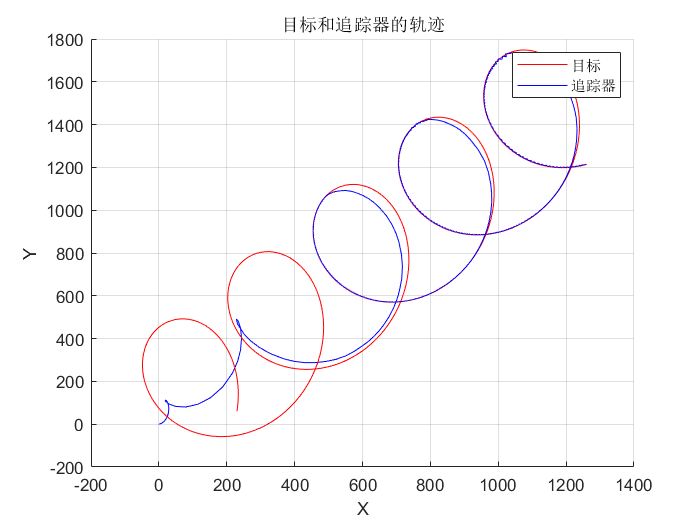
\includegraphics[width=5in]{pic/t6.png}
    \caption*{第六题轨迹}
\end{figure}
结论:最小追击速度: 292.35 米/秒;
追踪器在 14.96 秒内追上了目标。 

\quad 追踪器行进的轨迹长度: 8908.04 米;
目标行进的轨迹长度: 8399.64 米
\end{theorem}


%%%%%%%%%%%%%%%%%%%%%%%%%%%%%%%%%%%%%%%%%%%%%%%%%%%%%%%%%%
\subsection{第七题}

\begin{example}
    若跟踪器的运动速度$0\leq v \leq 400$ 米/秒的情况下,求能追上移动目标的最短追击
    时间;
\end{example}

\begin{theorem}
    通过遍历速度范围,逐步增加初始速度,寻找追踪器在30秒内追上目标的最优速度
    和最短追击时间。目标位置由参数化函数表示,代码在每次迭代中计算追踪器与
    目标在各个时间点的距离,若距离小于1米,则记录当前速度和追击时间,并更新最
    短时间和最优速度,最终输出最优速度和最短追击时间,并绘制目标和追踪器的轨迹图:
\begin{lstlisting}
% 目标位置的函数,假设从问题二中得到的参数已定义
targetX = @(t) a + b*t + A*cos(w1*t);
targetY = @(t) c + d*t + B*sin(w2*t);
targetZ = @(t) e + C*sin(w3*t);
% 设置初始速度范围
v_min = 0; % 初始速度
v_max = 400; % 最大速度
v_increment = 1; % 每次增加1米/秒
% 初始条件和时间区间
w0 = [0, 0, 0];
tspan = [0 30];
% 初始化最短时间变量
min_time = inf;
optimal_v = 0;
% 迭代寻找最小追击时间的速度
for v = v_min:v_increment:v_max
    odefun = @(t, w) [v * (targetX(t) - w(1)) / sqrt((targetX(t) - w(1))^2 ...
                     + (targetY(t) - w(2))^2 + (targetZ(t) - w(3))^2);
                        v * (targetY(t) - w(2)) / sqrt((targetX(t) - w(1))^2 ...
                     + (targetY(t) - w(2))^2 + (targetZ(t) - w(3))^2);
                        v * (targetZ(t) - w(3)) / sqrt((targetX(t) - w(1))^2 ...
                     + (targetY(t) - w(2))^2 + (targetZ(t) - w(3))^2)];
    [t, w] = ode45(odefun, tspan, w0);
    % 计算每一时间点上的距离
    distances = sqrt((targetX(t) - w(:,1)).^2 + (targetY(t) - w(:,2)).^2 ...
                    + (targetZ(t) - w(:,3)).^2);
    % 检查是否追上并计算追上时间
    if any(distances < 1) % 假设追上的条件是距离小于1米
        idx = find(distances < 1, 1, 'first');
        catch_time = t(idx);
        fprintf('追击时间: %.2f 秒\n', catch_time);
        % 更新最短时间和最优速度
        if catch_time < min_time
            min_time = catch_time;
            optimal_v = v;
        end
    end
end
% 输出结果
if min_time < inf
    fprintf('最优追击速度: %.2f 米/秒\n', optimal_v);
    fprintf('最短追击时间: %.2f 秒\n', min_time);
    % 以最优速度绘制轨迹图
    odefun = @(t, w) [optimal_v * (targetX(t) - w(1)) / sqrt((targetX(t) ... 
                     - w(1))^2 + (targetY(t) - w(2))^2 + (targetZ(t) - w(3))^2);
                        optimal_v * (targetY(t) - w(2)) / sqrt((targetX(t) ...
                     - w(1))^2 + (targetY(t) - w(2))^2 + (targetZ(t) - w(3))^2);
                        optimal_v * (targetZ(t) - w(3)) / sqrt((targetX(t) ... 
                     - w(1))^2 + (targetY(t) - w(2))^2 + (targetZ(t) - w(3))^2)];
    [t, w] = ode45(odefun, tspan, w0);
    figure;
    hold on;
    fplot3(targetX, targetY, targetZ, [0 30], 'r');
    plot3(w(:,1), w(:,2), w(:,3), 'b');
    title('目标和追踪器的轨迹');
    xlabel('X');
    ylabel('Y');
    zlabel('Z');
    legend('目标', '追踪器');
    grid on;
else
    fprintf('在最大速度 %d 米/秒内追踪器未能在30秒内追上目标。\n', v_max);
end    
\end{lstlisting}
\begin{figure}[h]
    \centering
    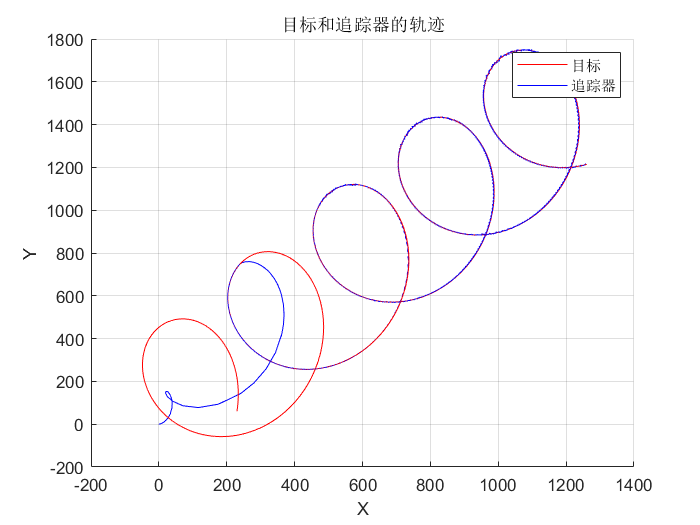
\includegraphics[width=5in]{pic/t7.png}
    \caption*{第七题轨迹}
\end{figure}
结论:最优追击速度: 400.00 米/秒;
最短追击时间: 8.60 秒
\end{theorem}
%%%%%%%%%%%%%%%%%%%%%%%%%%%%%%%%%%%%%%%%%%%%%%%%%%%%%%%%%%
\subsection{第八题}

\begin{example}
    若给出空间移动目标随时间移动的空间位置测量含噪数据文件
    (数据文件名data2.txt,数据格式$[t,x_1(t),y_1(t),z_1(t)]$)
    如何处理上述问题?并给出相应的结果。  
\end{example}


\begin{theorem}
    首先对含噪声数据进行降噪处理:
\begin{lstlisting}
% 加载含噪声数据
data = readmatrix('data2.txt');
t2 = data(:, 1);  % 时间
x = data(:, 2);  % x坐标
y = data(:, 3);  % y坐标
z = data(:, 4);  % z坐标
% 使用局部加权回归平滑对数据去噪处理
x2 = smooth(t, x, 0.1, 'rloess');  
y2 = smooth(t, y, 0.1, 'rloess');
z2 = smooth(t, z, 0.1, 'rloess');
\end{lstlisting}

\newpage
下面是除噪后数据与无噪声数据的分量对比:
\begin{figure}[h]
    \centering
    \nonumber
    \subfigure{
    \begin{minipage}[t]{0.32\linewidth}
    \centering
    \nonumber
    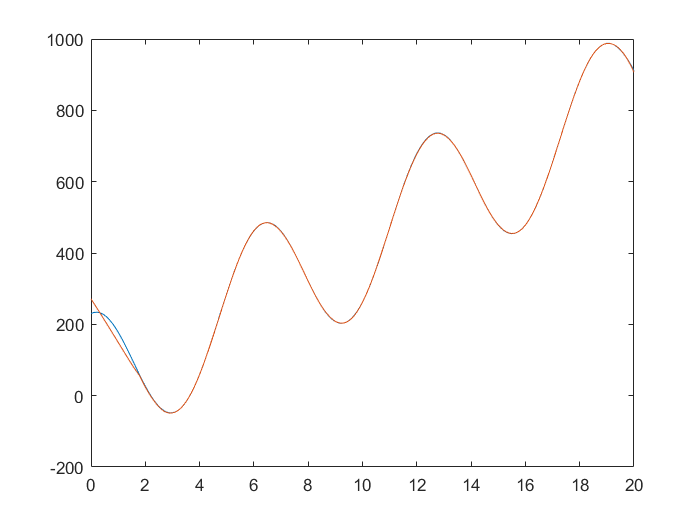
\includegraphics[width=2in]{pic/compare_x.png}
    \caption*{x分量}
    \end{minipage}}
    \subfigure{
    \begin{minipage}[t]{0.32\linewidth}
    \centering
    \nonumber
    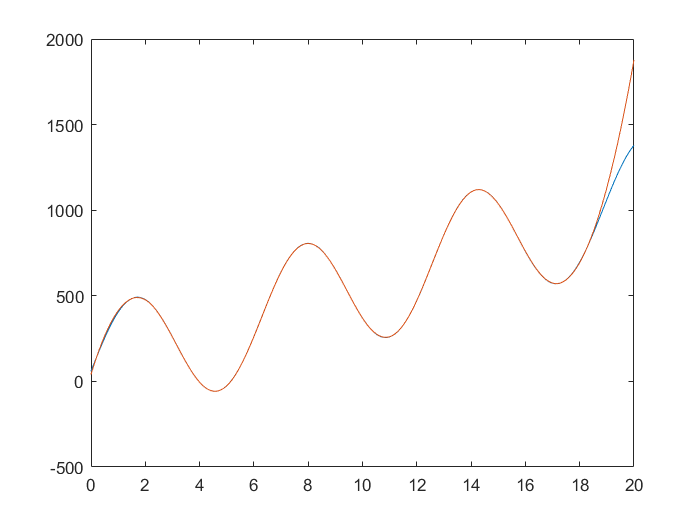
\includegraphics[width=2in]{pic/compare_y.png}
    \caption*{y分量}
    \end{minipage}}
    \subfigure{
    \begin{minipage}[t]{0.32\linewidth}
    \centering
    \nonumber
    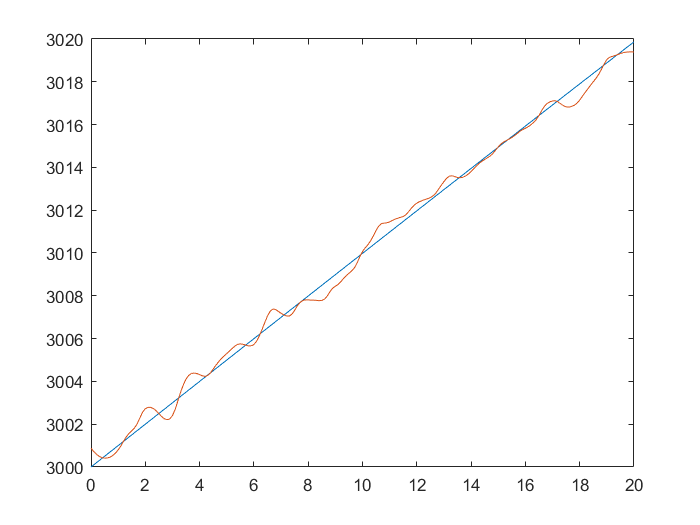
\includegraphics[width=2in]{pic/compare_z.png}
    \caption*{z分量}
    \end{minipage}}
    \caption*{红色为含噪声数据,蓝色为无噪声数据}
\end{figure}

接下来,我们使用$(x_2(t),y_2(t),z_2(t))$来进行后续的分析。使用第二题的方法
拟合数据,得到的结果对比如下:(括号内第一项为data1拟合结果,第二项为data2拟合结果)
\begin{table}[h]
    \centering
    \begin{tabular}{|c|c|c|c|}
        \hline
        $a$ & $b$ & $A$ & $\omega_1$ \\
        \hline
        (30.000,26.155) & (40.000,40.267) & (200.000,199.249) & (1.000,1.000) \\
        \hline
        $c$ & $d$ & $B$ & $\omega_2$ \\
        \hline
        (60.000,33.008) & (50.000,53.899) & (350.000,373.69) & (1.000,1.004) \\
        \hline
        $e$ & $C$ & $\omega_3$ & {} \\
        \hline
        (3.0000.000,3000.124) & (1.000.105,51.010) & (0.010,0.019) & {} \\
        \hline
    \end{tabular}
\end{table}

由于接下来的代码结构和上面3-7问的一样,所以下面忽略代码,只展示结果:
\begin{itemize}
    \item 拟合最大速度: 434.083092 米/秒;拟合最小速度: 157.361971 米/秒
    \item 追踪器在$v=290,200 m/s$时在 30 秒内未能追上目标
    \item 最小追击速度: 311.05 米/秒,此时追踪器在 20.97 秒内追上了目标。
    追踪器行进的轨迹长度: 9478.01 米;目标行进的轨迹长度: 8803.99 米。
    \item 最优追击速度: 400.00 米/秒;对应的最短追击时间: 8.66 秒
\end{itemize}


\newpage
下面的图片是除躁数据输出的结果图:
\begin{figure}[h]
    \centering
    \nonumber
    \subfigure{
    \begin{minipage}[t]{0.45\linewidth}
    \centering
    \nonumber
    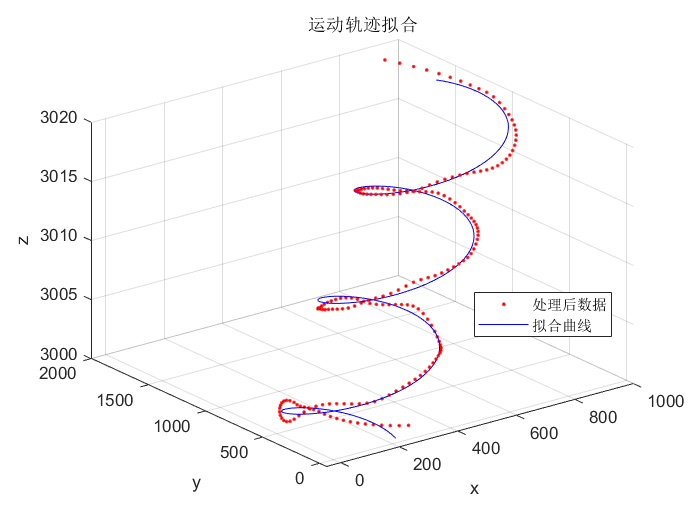
\includegraphics[width=3in]{pic/8fit.png}
    \caption*{拟合轨迹}
    \end{minipage}}
    \subfigure{
    \begin{minipage}[t]{0.45\linewidth}
    \centering
    \nonumber
    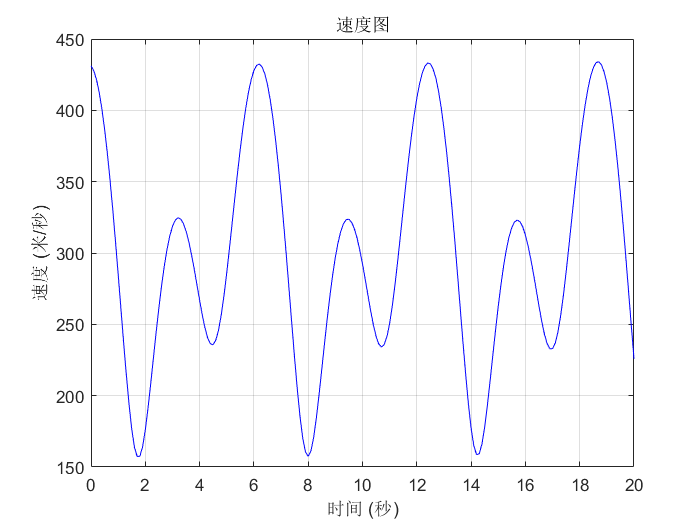
\includegraphics[width=3in]{pic/8fit_speed.png}
    \caption*{拟合速度}
    \end{minipage}}

    \subfigure{
    \begin{minipage}[t]{0.3\linewidth}
    \centering
    \nonumber
    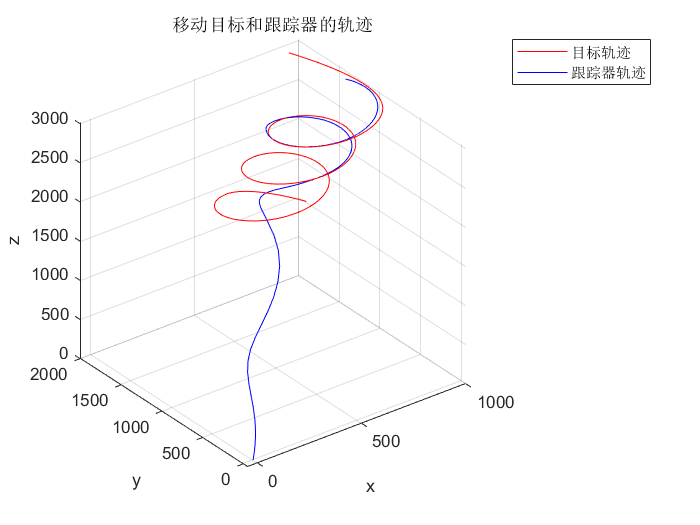
\includegraphics[width=2in]{pic/8t3.png}
    \caption*{第三题轨迹}
    \end{minipage}}
    \subfigure{
    \begin{minipage}[t]{0.3\linewidth}
    \centering
    \nonumber
    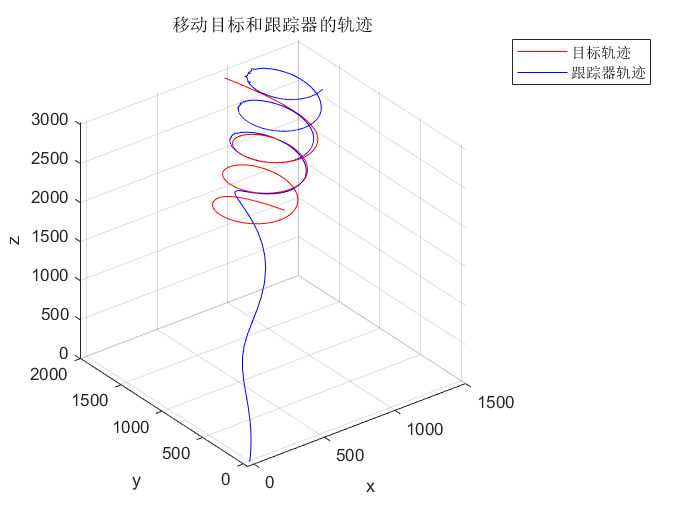
\includegraphics[width=2in]{pic/8t4.png}
    \caption*{第四题轨迹}
    \end{minipage}}
    \subfigure{
    \begin{minipage}[t]{0.3\linewidth}
    \centering
    \nonumber
    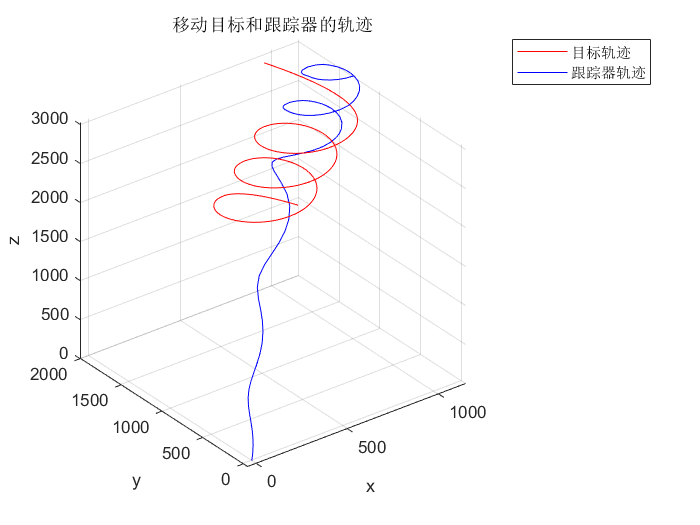
\includegraphics[width=2in]{pic/8t5.png}
    \caption*{第五题轨迹}
    \end{minipage}}

    \subfigure{
    \begin{minipage}[t]{0.45\linewidth}
    \centering
    \nonumber
    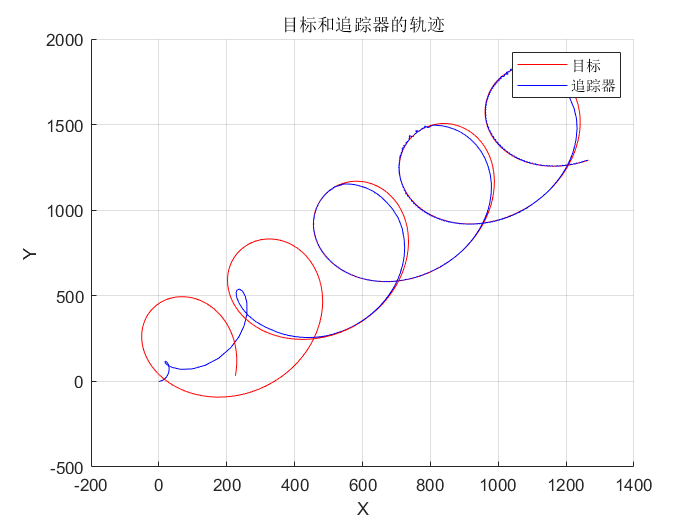
\includegraphics[width=3in]{pic/8t6.png}
    \caption*{第六题轨迹}
    \end{minipage}}
    \subfigure{
    \begin{minipage}[t]{0.45\linewidth}
    \centering
    \nonumber
    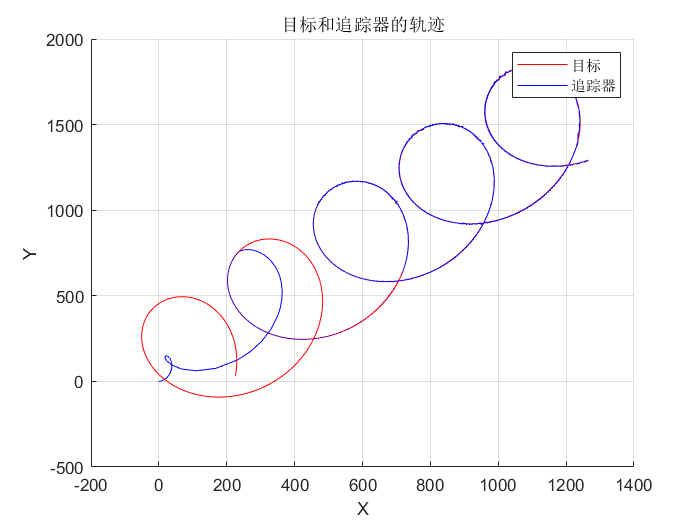
\includegraphics[width=3in]{pic/8t7.png}
    \caption*{第七题轨迹}
    \end{minipage}}
\end{figure}

\end{theorem}

\end{document}
